% !TEX root = ../main.tex
\chapter{Results and Discussion}\label{ch:results}
\section{Background}
loading, cleaning data, description data

\section{Solution Groups}

\section{Scoring Groups}

\section{Solution Distance matrix}
The first avenue of analysis, after constructing descriptive data, was to look at the relationship strategies have with each other.
A distance matrix shows how much an opponent differs from every other, if 2 sequences are similar with respect to the distance function then they will score lower than 2 sequences that are more distinct.
Certain distance functions have been selected because of their connotations.

\paragraph{Hamming Distance}
$$$$

\paragraph{Cosine Distance}
$$ d(O_i,O_j) = cos(\theta) = \frac{\textbf{A} \cdot \textbf{B}}{|| \textbf{A} || \; || \textbf{B} ||} $$
The cosine of two vectors constructed by using the dot product formula as shown above.
Figure~\ref{fig:cosine} shows an interpretation of this in 2 dimensions, in our interpretation each dimension represents a sequence element so we are working in $\mathbb{R}^{200}$ with every value taking a $1$(C) or a $0$(D).
\begin{figure}[h]
    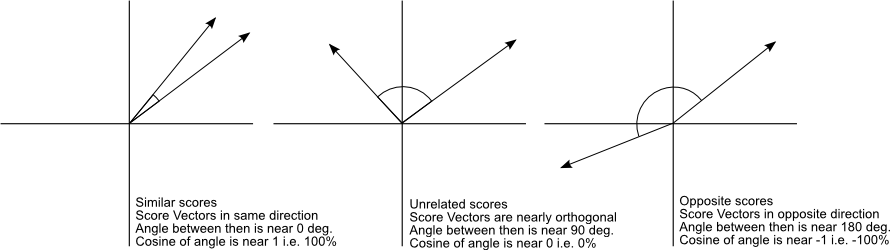
\includegraphics[width=1.0\textwidth, center]{./img/examples/cosinesimilarity.png}
    \caption{An Example of 2d cosine similarity~\cite{Perone2013blog}}\label{fig:cosine}
\end{figure}
Figure~\ref{fig:dist_cos} shows the distance matrix generated from the data files using code 




\begin{figure}[ht]
        \centering
        \begin{minipage}{0.48\textwidth}
            \centering
            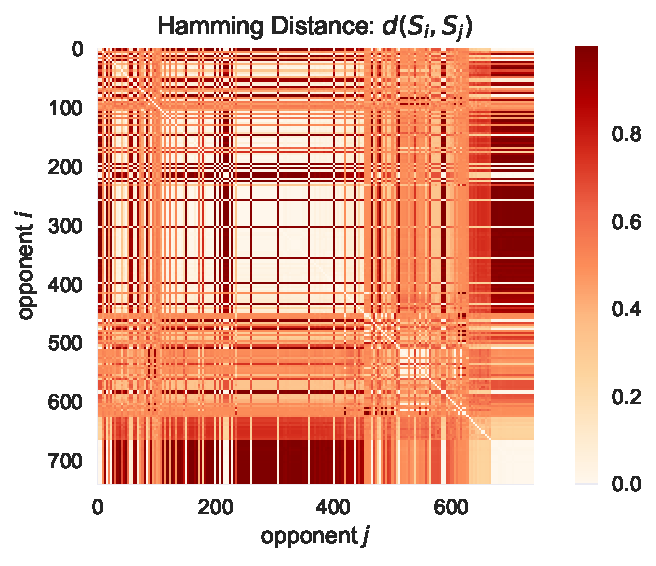
\includegraphics[width=1.0\textwidth, center]{./img/dist_matrix/dist_ham.pdf}
            \caption{}\label{fig:dist_ham}
        \end{minipage}\hfill
        \begin{minipage}{0.48\textwidth}
            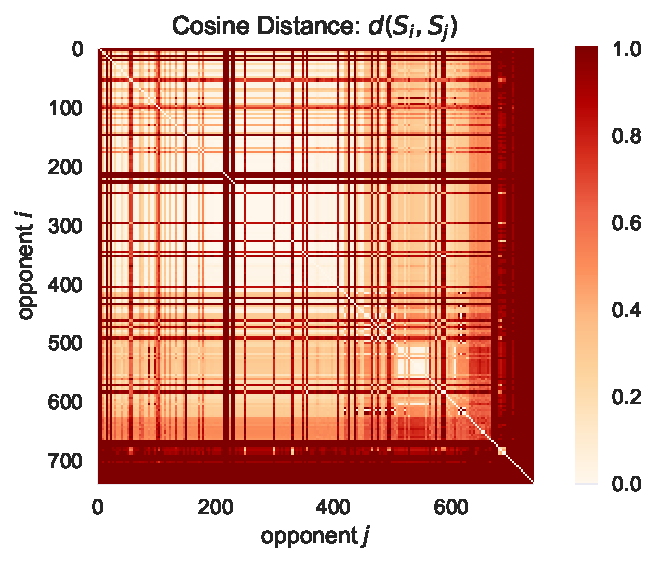
\includegraphics[width=1.0\textwidth]{./img/dist_matrix/dist_cos.pdf} 
            \caption{}\label{fig:dist_cos}
        \end{minipage}
    \end{figure}

\section{Clustering Analysis}